%% Los cap'itulos inician con \chapter{T'itulo}, estos aparecen numerados y
%% se incluyen en el 'indice general.
%%
%% Recuerda que aqu'i ya puedes escribir acentos como: 'a, 'e, 'i, etc.
%% La letra n con tilde es: 'n.
\chapter{Resultados}
\section{Paquete de R \emph{geneticae}}

El paquete \emph{geneticae} ofrece funciones para el análisis de datos de etapas avanzadas de programas de mejoramiento, donde se evalúan pocos genotipos. Para instalarlo se deben utilizar las siguientes sentencias:

\begin{lstlisting}
install.packages("devtools")
library(devtools)
install_github("jangelini/geneticae")
\end{lstlisting}

Una vez que se instala el paquete geneticae, se debe cargar en la sesion de R:

\begin{lstlisting}
library(geneticae)
\end{lstlisting}


Se puede obtener información detallada sobre las funciones del paquete geneticae de los archivos de ayuda mediante \emph{help (package = "geneticae")}.  La ayuda para una función, por ejemplo, imputación, en una sesión R se puede obtener usando \emph{?imputation} o \emph{help(imputation)}.


\subsection{Conjuntos de datos incluidos}

El paquete geneticae proporciona dos conjuntos de datos para ilustrar la metodología incluida para analizar los datos MET.

\begin{itemize}
\item yan.winterwheat dataset: rendimiento de 18 variedades de trigo de invierno cultivadas en nueve ambientes en Ontario en 1993. No hay réplicas disponibles en los datos. Este conjunto de datos se obtuvo del paquete agridat.

\begin{lstlisting}
library(geneticae)
data(yan.winterwheat)
dat_yan <- yan.winterwheat
head(dat_yan)
\end{lstlisting}

\begin{verbatim}
##   gen  env yield
## 1 Ann BH93 4.460
## 2 Ari BH93 4.417
## 3 Aug BH93 4.669
## 4 Cas BH93 4.732
## 5 Del BH93 4.390
## 6 Dia BH93 5.178
\end{verbatim}

\item plrv dataset: rendimiento, peso de planta y parcela de 28 clones de la población del virus del enrollamiento de la papa (PLRV) evaluada en seis entornos. Las réplicas están disponibles en los datos. Este conjunto de datos se obtuvo del paquete agricolae.

\begin{lstlisting}
data(plrv)
dat_rep <- plrv
head(dat_rep)
\end{lstlisting}


\begin{verbatim}
##   Genotype Locality Rep WeightPlant WeightPlot    Yield
## 1   102.18     Ayac   1   0.5100000       5.10 18.88889
## 2   104.22     Ayac   1   0.3450000       2.76 12.77778
## 3   121.31     Ayac   1   0.5425000       4.34 20.09259
## 4   141.28     Ayac   1   0.9888889       8.90 36.62551
## 5   157.26     Ayac   1   0.6250000       5.00 23.14815
## 6    163.9     Ayac   1   0.5120000       2.56 18.96296
\end{verbatim}
\end{itemize}
 
\subsection{Funciones incluidas}

\textbf{Modelo de regresión por sitio}

Para ejecutar la función \emph{GGEmodel}, se debe proporcionar un conjunto de datos con genotipos, ambientes, repeticiones (si hay disponibles), el fenotipo observado y los nombres de las variables en el archivo de entrada. Además, se debe indicar el método de centrado, escala y SVD.

Cuando no hay repeticiones disponibles en el conjunto de datos, como es el caso del conjunto de datos yan.winterwheat, el modelo GGE se indica de la siguiente manera:


\begin{lstlisting}
GGE1 <- GGEmodel(dat_yan, genotype = "gen", environment = "env", 
response = "yield", centering = "tester")
\end{lstlisting}


Sin embargo, en el caso de que haya repeticiones disponibles, como el conjunto de datos plrv, se indica de la siguiente manera:


\begin{lstlisting}
GGE1_rep <- GGEmodel(dat_rep, genotype = "Genotype", environment = "Locality", 
response = "Yield", rep = "Rep", centering = "tester")
\end{lstlisting}


La salida de la función GGEmodel es una lista con los siguientes elementos:


\begin{itemize}
\item coordgenotype: trazado de coordenadas para genotipos de todos los componentes.
\item coordenviroment: trazado de coordenadas para entornos de todos los componentes.
\item valores propios: vector de valores propios de cada componente.
\item vartotal: varianza general.
\item varexpl: porcentaje de varianza explicado por cada componente.
\item labelgen: nombres de genotipo.
\item labelenv: nombres de entorno.
\item ejes: etiquetas de eje.
\item Datos: datos de entrada escalados y centrados.
\item centrado: nombre del método de centrado.
\item escala: nombre del método de escala.
\item SVP: nombre del método SVP.
\end{itemize}


Por ejemplo, para el conjunto de datos yan.winterwheat:


\begin{lstlisting}
names(GGE1)
\end{lstlisting}

\begin{verbatim}
##  [1] "coordgenotype"   "coordenviroment" "eigenvalues"    
##  [4] "vartotal"        "varexpl"         "labelgen"       
##  [7] "labelenv"        "labelaxes"       "Data"           
## [10] "centering"       "scaling"         "SVP"
\end{verbatim}

\textbf{Biplot GGE}

Para ejecutar la función \emph{GGEPlot}, se requiere un objeto de la clase \emph{GGEmodel}. La salida es un biplot construido a través de los componentes principales generados por \emph{GGEmodel}.

Los diferentes biplots que se pueden obtener usando la función \emph{GGEPlot} se muestran usando el conjunto de datos yan.winterwheat.


\begin{itemize}
\item Biplot básico, se obtiene indicando type = "Biplot".

\begin{lstlisting}
GGEPlot(GGE1, type = "Biplot")
\end{lstlisting}

\begin{figure}[h]
	\begin{center}
		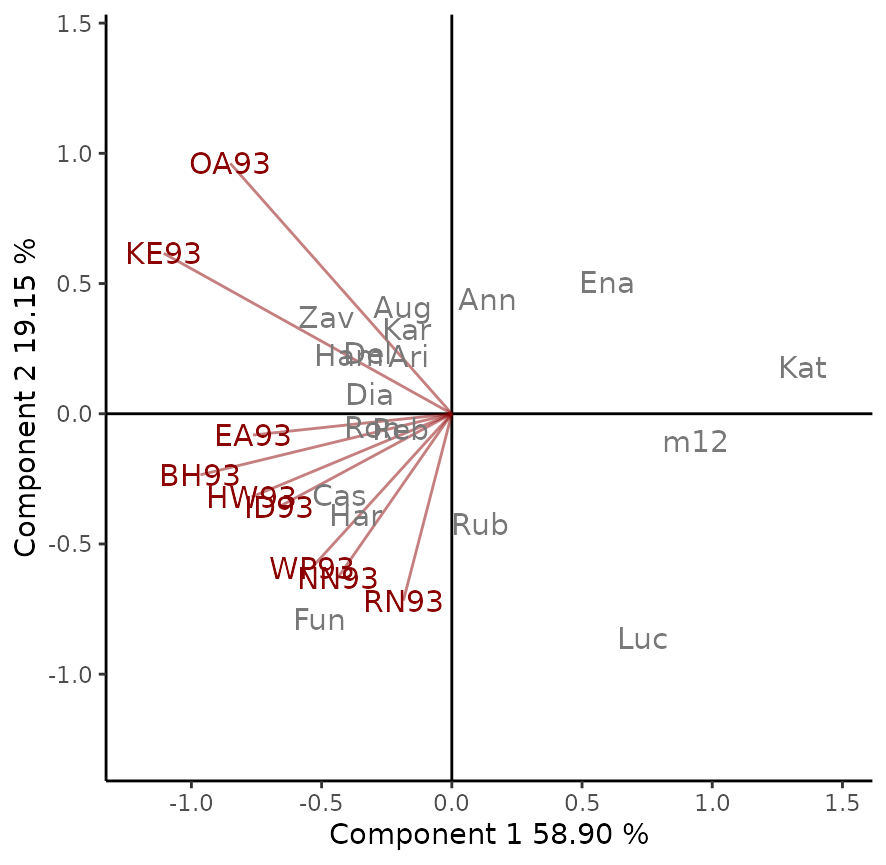
\includegraphics[width=10cm]{./Graficos/GGE_BIPLOT.png}
	\end{center}
	\caption{Biplot básico obtenido de la función \emph{GGEPlot}}
\end{figure}

\item Biplot básico, se obtiene indicando type = "Biplot".

\item Ranking de los cultivares en función de su rendimiento en cualquier ambiente dado se obtiene indicando type="Selected Environment" y el nombre del ambiente para examinarse selectedE = "OA93".

\begin{lstlisting}
GGEPlot(GGE1, type = "Selected Environment", selectedE = "OA93")
\end{lstlisting}


\begin{figure}[h]
	\begin{center}
		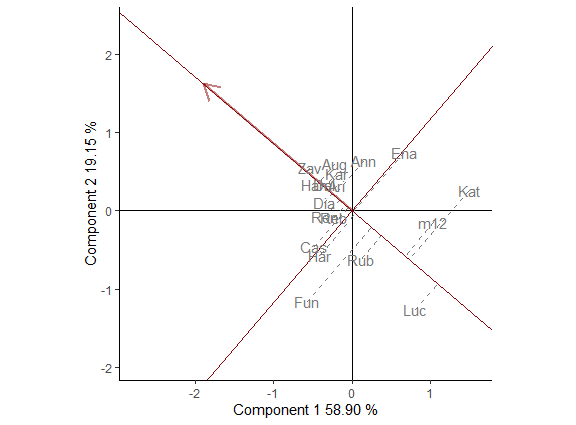
\includegraphics[width=10cm]{./Graficos/SelectedEnvironment.png}
	\end{center}
	\caption{Ranking de cultivares para un ambiente determinado obtenido de la función \emph{GGEPlot}}
\end{figure}


\item Ranking de los ambientes en función del rendimiento relativo de cualquier cultivar determinado se obtiene indicando  type="Selected Genotype" y el nombre del ambiente para examinarse selectedG = "Kat".

\begin{lstlisting}
GGEPlot(GGE1, type = "Selected Genotype", selectedG = "Kat")
\end{lstlisting}

\begin{figure}[h]
	\begin{center}
		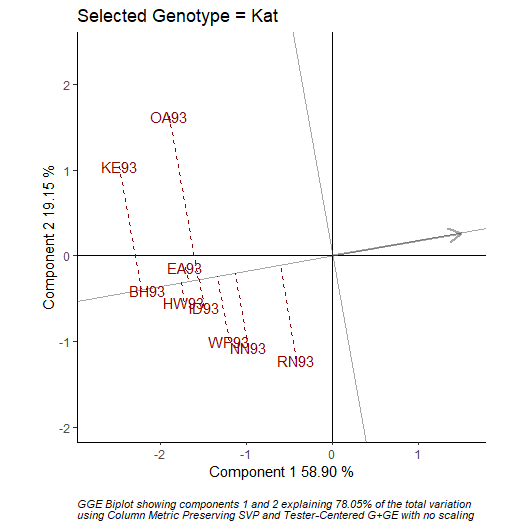
\includegraphics[width=10cm]{./Graficos/SelectedGenotype.png}
	\end{center}
	\caption{Ranking de ambientes para cultivar determinado obtenido de la función \emph{GGEPlot}}
\end{figure}


\item Relación entre ambientes, se obtiene indicando type="Relationship Among Environments".

\begin{lstlisting}
GGEPlot(GGE1, type = "Relationship Among Environments")
\end{lstlisting}

\begin{figure}[h]
	\begin{center}
		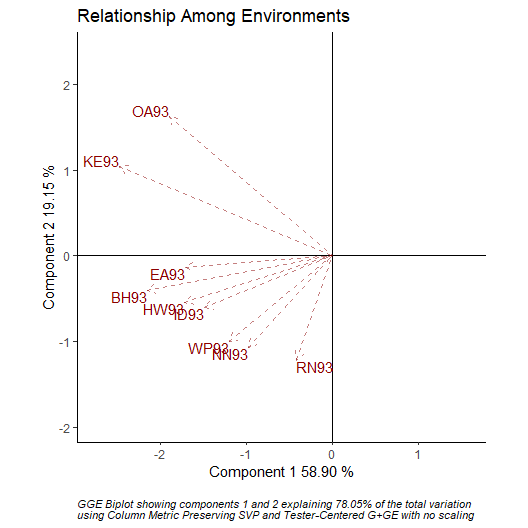
\includegraphics[width=10cm]{./Graficos/RelationshipAmongEnvironments.png}
	\end{center}
	\caption{Relación entre ambientes obtenido de la función \emph{GGEPlot}}
\end{figure}

\item Comparación entre dos genotipos se obtiene indicando type = "Comparison of Genotype" y los genotipos para comparar selectedG1 = "Kat" con selectedG2 = "Cas".

\begin{lstlisting}
GGEPlot(GGE1, type = "Comparison of Genotype", selectedG1 = "Kat", selectedG2 = "Cas")
\end{lstlisting}

\begin{figure}[h]
	\begin{center}
		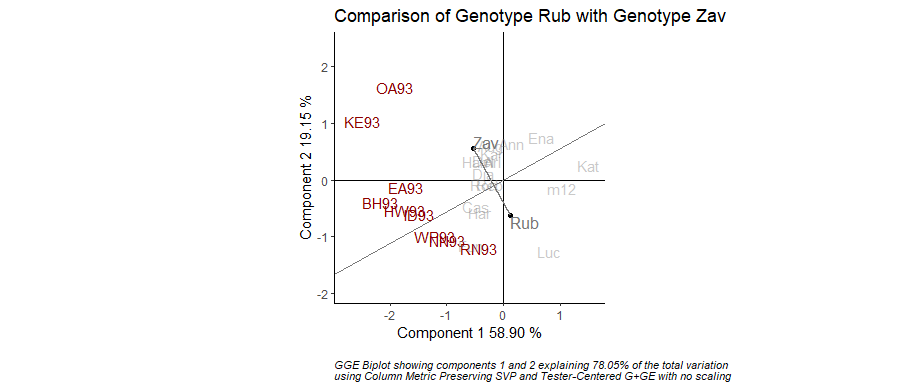
\includegraphics[width=10cm]{./Graficos/ComparisonofGenotype.png}
	\end{center}
	\caption{Comparación entre dos genotipos obtenido de la función \emph{GGEPlot}}
\end{figure}


\item Identificación del mejor cultivar en cada ambiente indicando type = "Which Won Where/What".

\begin{lstlisting}
GGEPlot(GGE1, type = "Which Won Where/What")
\end{lstlisting}

\begin{figure}[h]
	\begin{center}
		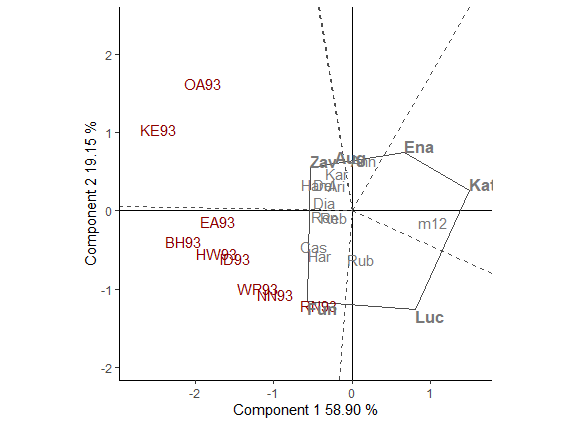
\includegraphics[width=10cm]{./Graficos/WhichWonWhereWhat.png}
	\end{center}
	\caption{Identificación del mejor cultivar en cada ambiente a partir de la función \emph{GGEPlot}}
\end{figure}



\item Evaluación de los ambientes basados tanto en la capacidad de discriminación como en la representatividad indicando type = "Which Won Where/What".

\begin{lstlisting}
GGEPlot(GGE1, type = "Discrimination vs. representativeness")
\end{lstlisting}

\begin{figure}[h]
	\begin{center}
		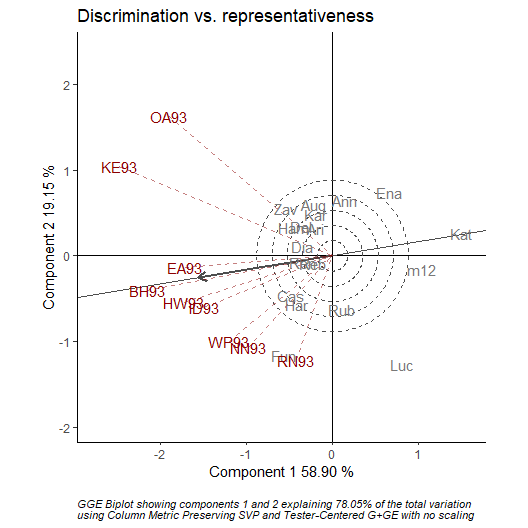
\includegraphics[width=10cm]{./Graficos/Discriminationvsrepresentativeness.png}
	\end{center}
	\caption{Evaluación de los ambientes basados tanto en la capacidad de discriminación y representatividad a partir de la función \emph{GGEPlot}}
\end{figure}



\item Clasificación de ambientes con respecto al ambiente ideal, indicando type="Ranking Environments".

\begin{lstlisting}
GGEPlot(GGE1, type = "Ranking Environments")
\end{lstlisting}

\begin{figure}[h]
	\begin{center}
		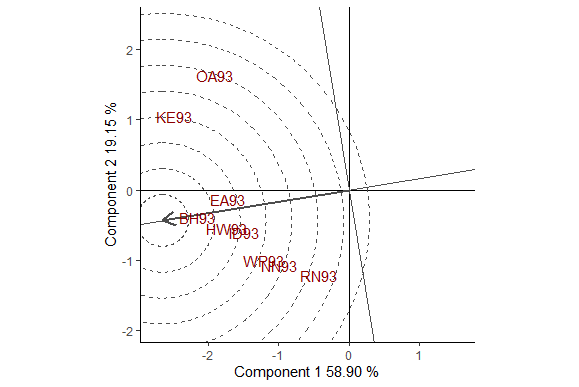
\includegraphics[width=10cm]{./Graficos/RankingEnvironments.png}
	\end{center}
	\caption{Clasificación de ambientes con respecto al ambiente ideal a partir de la función \emph{GGEPlot}}
\end{figure}


\item Clasificación de genotipos con respecto al genotipo ideal, indicando type = "Ranking Genotypes".

\begin{lstlisting}
GGEPlot(GGE1, type = "Ranking Genotypes")
\end{lstlisting}

\begin{figure}[h]
	\begin{center}
		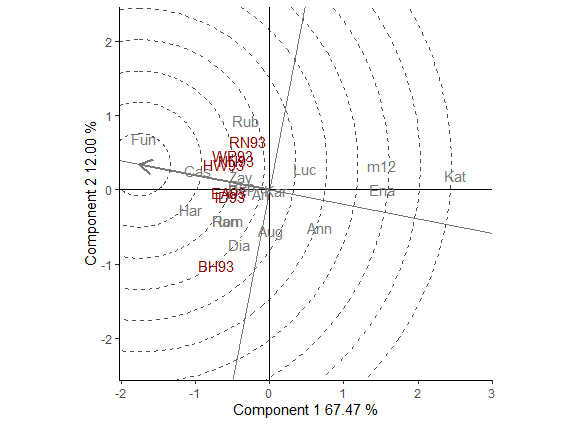
\includegraphics[width=10cm]{./Graficos/RankingGenotypes.png}
	\end{center}
	\caption{Clasificación de genotipos con respecto al genotipo ideal a partir de la función \emph{GGEPlot}}
\end{figure}

\item Evaluación de los cultivares con base en el rendimiento promedio y la estabilidad, indicando type = "Mean vs. Stability".

\begin{lstlisting}
GGEPlot(GGE1, type = "Mean vs. Stability")
\end{lstlisting}

\begin{figure}[h]
	\begin{center}
		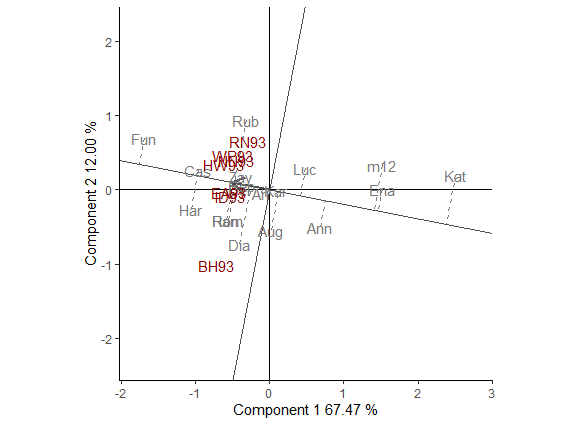
\includegraphics[width=10cm]{./Graficos/MeanvsStability.png}
	\end{center}
	\caption{Evaluación de los cultivares con base en el rendimiento promedio y la estabilidad a partir de la función \emph{GGEPlot}}
\end{figure}

\end{itemize}


\textbf{Classic AMMI model}

Para ejecutar la función rAMMI, como en la función GGEmodel, se debe proporcionar un conjunto de datos con genotipo, entorno, repeticiones (si las hay) y la variable de respuesta. Se debe indicar el nombre de las columnas que contienen genotipo, entorno, repeticiones y la respuesta. La salida es un biplot.

A continuación se muestra el biplot GE obtenido del modelo AMMI clásico obtenido con el conjunto de datos yan.winterwheat.

\begin{lstlisting}
rAMMI(dat_yan, genotype = "gen", environment = "env", response = "yield", type = "AMMI")
\end{lstlisting}

\begin{figure}[h]
	\begin{center}
		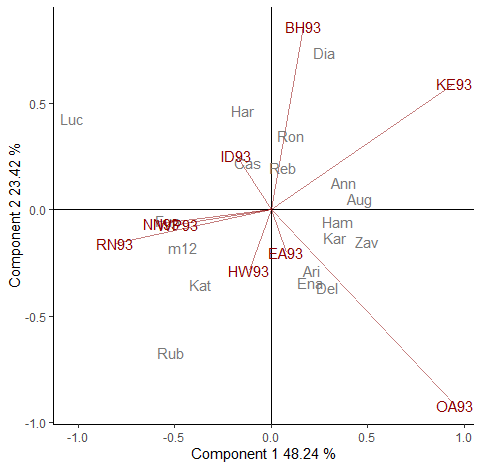
\includegraphics[width=10cm]{./Graficos/AMMI.png}
	\end{center}
	\caption{Biplot GE obtenido del modelo clasico AMMI}
\end{figure}

\textbf{Robust AMMI model}

Los biplots de los cinco modelos AMMI robustos propuestos por Rodrigues et al. (2015), usando el conjunto de datos yan.winterwheat se muestran a continuación.

\begin{itemize}

\item  type = "rAMMI"

\begin{lstlisting}
rAMMI(dat_yan, genotype = "gen", environment = "env", response = "yield", type = "rAMMI")
\end{lstlisting}

\begin{figure}[h]
	\begin{center}
		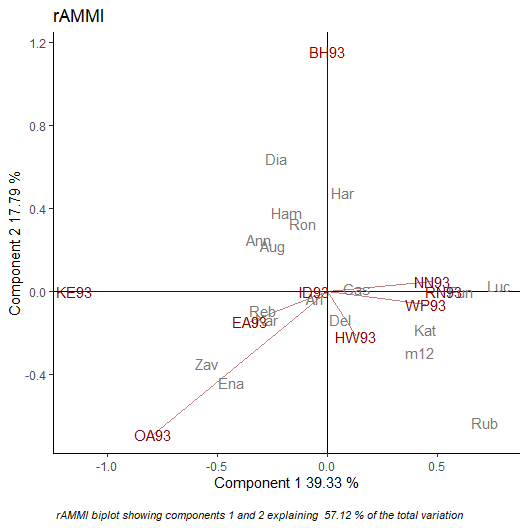
\includegraphics[width=10cm]{./Graficos/rAMMI.png}
	\end{center}
	\caption{Biplot GE obtenido del modelo robusto rAMMI}
\end{figure}


\item  type = "hAMMI"

\begin{lstlisting}
rAMMI(dat_yan, genotype = "gen", environment = "env", response = "yield", type = "hAMMI")
\end{lstlisting}

\begin{figure}[h]
	\begin{center}
		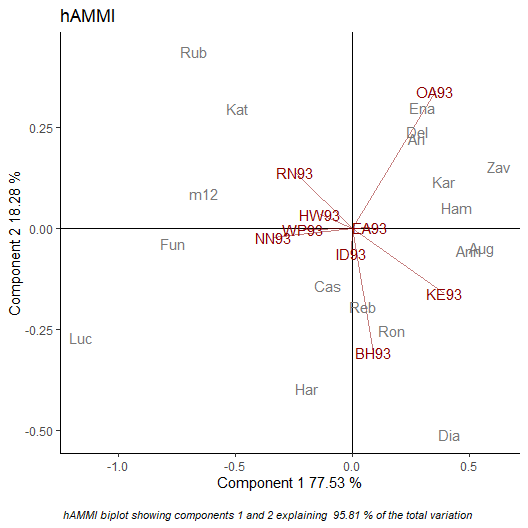
\includegraphics[width=10cm]{./Graficos/hAMMI.png}
	\end{center}
	\caption{Biplot GE obtenido del modelo robusto hAMMI}
\end{figure}


\item  type = "gAMMI"

\begin{lstlisting}
rAMMI(dat_yan, genotype = "gen", environment = "env", response = "yield", type = "gAMMI")
\end{lstlisting}

\begin{figure}[h]
	\begin{center}
		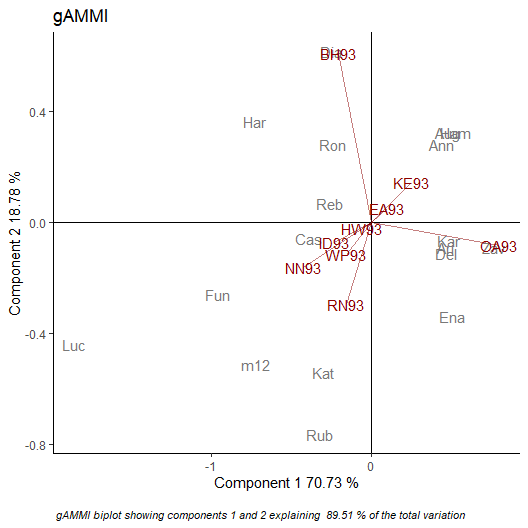
\includegraphics[width=10cm]{./Graficos/gAMMI.png}
	\end{center}
	\caption{Biplot GE obtenido del modelo robusto hAMMI}
\end{figure}



\item  type = "lAMMI"

\begin{lstlisting}
rAMMI(dat_yan, genotype = "gen", environment = "env", response = "yield", type = "lAMMI")
\end{lstlisting}


\begin{figure}[h]
	\begin{center}
		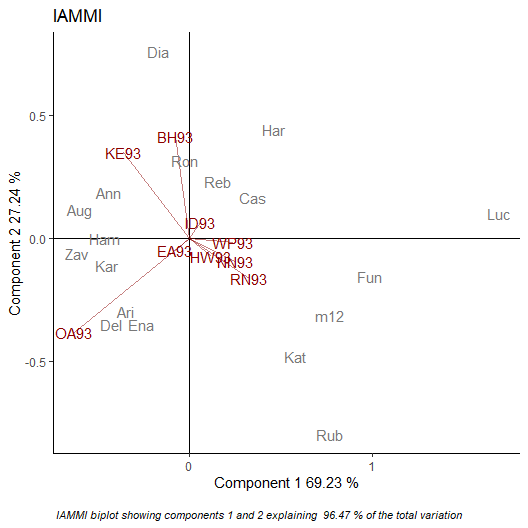
\includegraphics[width=10cm]{./Graficos/lAMMI.png}
	\end{center}
	\caption{Biplot GE obtenido del modelo robusto hAMMI}
\end{figure}


\item  type = "ppAMMI"
\begin{lstlisting}
rAMMI(dat_yan, genotype = "gen", environment = "env", response = "yield", type = "ppAMMI")
\end{lstlisting}


\begin{figure}[h]
	\begin{center}
		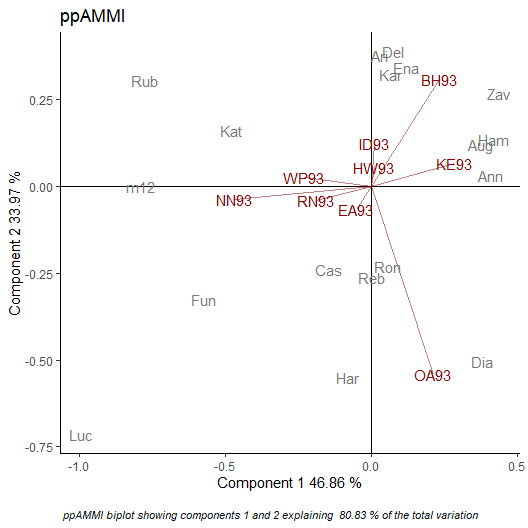
\includegraphics[width=10cm]{./Graficos/ppAMMI.png}
	\end{center}
	\caption{Biplot GE obtenido del modelo robusto hAMMI}
\end{figure}

\end{itemize}
\section{Geneticae Shiny Web App}

En primer lugar se debe cargar el paquete Shiny como primera línea del script:

\begin{lstlisting}[frame=single]
library(shiny) 
\end{lstlisting}

La funcion ui contiene todas las indicaciones para construir la interfaz del usuario. Estas instrucciones se pueden agrupar con respecto a los siguientes aspectos:
\begin{enumerate}
\item La estructura de la aplicación: Por defecto, las aplicaciones hechas con Shiny tienen un título, un panel lateral y un panel principal que se indican con las funciones headerPanel(), sidebarPanel() y mainPanel().
\item Los inputs: La reactividad de la aplicación toma como punto de partida los inputs que son los campos en los que dejamos libertad al usuario para elegir diferentes valores a través de los widgets. Hay diferentes tipos de widgets como los que reciben valores numéricos, texto, listas desplegables, etc. En nuestra aplicación, hemos incluido el widget sliderInput() que inserta una barra deslizable y permite elegir un valor de r entre -1 y 1. El valor seleccionado pasará a server.R bajo el nombre de r\$input donde el identificador "r" aparece como el primer argumento de la función sliderInput().
\item Los outputs: La reactividad de la aplicación fructifica en los outputs que son los resultados (valores numéricos, tablas, gráficos) que recibe la interfaz desde el server.R. En nuestro caso, el resultado es un gráfico y se inserta con la función
plotOutput().
\end{enumerate}

Además de las funciones citadas, el usuario puede encontrar las siguientes:
\begin{enumerate}
\item  h5(): Contenido de texto con diferentes tamaños. Otros tamaños son h1(), h2(), h3() y h4().
\item p(): Bloques de texto con diferentes componentes.
\item img(): Imagen (los archivos de las imágenes incluidas deben estar dentro del subdirectorio www).
\end{enumerate}

El archivo server.R realiza las operaciones necesarias hasta obtener los outputs que envía como resultado a ui.R. Como hemos mencionado anteriormente, nuestra aplicación depende del valor del input r\$input. Este archivo comienza de nuevo cargando el paquete Shiny y todos los necesarios para realizar los cálculos correspondientes. A excepción de las funciones definidas en R que sean necesarias para el tratamiento de los inputs, los cálculos concretos que deben "reaccionar" a las decisiones de los usuarios están incluidos dentro de  


Las funciones ui y server de nuestra aplicación se encuentra en el apéndice B.


